\documentclass{article}


% if you need to pass options to natbib, use, e.g.:
%     \PassOptionsToPackage{numbers, compress}{natbib}
% before loading neurips_2021

% ready for submission
\usepackage[final]{neurips_2021}

% to compile a preprint version, e.g., for submission to arXiv, add add the
% [preprint] option:
%     \usepackage[preprint]{neurips_2021}

% to compile a camera-ready version, add the [final] option, e.g.:
%     \usepackage[final]{neurips_2021}

% to avoid loading the natbib package, add option nonatbib:
%    \usepackage[nonatbib]{neurips_2021}

\usepackage[utf8]{inputenc} % allow utf-8 input
\usepackage[T1]{fontenc}    % use 8-bit T1 fonts
\usepackage{hyperref}       % hyperlinks
\usepackage{url}            % simple URL typesetting
\usepackage{booktabs}       % professional-quality tables
\usepackage{amsfonts}       % blackboard math symbols
\usepackage{nicefrac}       % compact symbols for 1/2, etc.
\usepackage{microtype}      % microtypography
\usepackage{xcolor}         % colors
\usepackage{graphicx}

\title{Generation of Dashcam Footage via a beta-VAE-GAN - Analysis and Preliminary work for an end-to-end AV controller}
\author{
Alex Richardson \\
  Department of Computer Science\\
  Vanderbilt University\\
  \textit{william.a.richardson@vanderbilt.edu}
}
\begin{document}
\maketitle

\section{Introduction and Project Aims}
\subsection{Introduction}
 This work summarizes the early efforts of attempting to "train" a "data-driven" AV simulator via training an AV end-to-end controller model that simultaneously "hallucinates" the simulation while issuing driving commands. This in many ways is based on a similar but much simpler work done by Comma.Ai several years ago \cite{santana2016learning}. The overall model is as follows. Let $t_{t}$ be the current time in which the model is operating. We use a convolutional hybrid beta-VAE-GAN to encode the last two frames of dashcam footage (at $t_{t - 1}$ and $t_{t}$ respectively) into a latent space. The AV controller, which will be a standard feed-forward neural network, will accept as input this latent space, current GPS position (not encoded into the latent space) and the desired GPS destination. In turn, this controller will output new latents, which are then decoded using the VAE to generate an hallucinated predicted dashcam frame for time $t_{t + 1}$, along with new specified IMU behavior. Respectively, these represent the controller's prediction for the surrounding environment (or "simulation") and driving commands. This preliminary work covers the training and analysis around the beta-VAE-GAN, in particular of the beta hyperparameter - which in theory would allow us to understand if the encoder-decoder disentangling variables such as daytime conditions, among other variables. Our primary experiment involved heuristic sweeping of the beta hyperparameter at 1,10,100, and 250 respectively with examination of changes to each latent variable at those hyperparameter settings to determine the degree of entanglement subjectively. Our analysis indicates that the beta-VAE-GAN scheme, once made trainable with various augmentations to the Comma.Ai's loss functions, was unable to properly disentangle the variables in the latent space and produced mode collapse - which indicates that this latent space would likely not be very usable for an end-to-end AV controller. This mode collapse was initially obvious from an immediate comparison of the initial image and its reconstruction, and while it was subjectively reduced, it was still apparent upon a closer analysis of the latent variables. More work will be needed to create a latent space encoding that creates a more acceptable degree of disentanglement.
 \subsection{Hypotheses}
 \begin{enumerate}
     \item The beta-VAE-GAN is capable of reconstruction of dashcam footage, in the sense that the reconstructions will improve over the epochs subjectively and at least vaguely resemble the original image. 
    \item Increasing the beta parameter, which weighs the KL-divergence loss for the encoder, will result in more and more disentangling of the latent variables.
\end{enumerate}
Combined, these two hypotheses, if not disproven, would set the stage for an end-to-end AV controller scheme, based off of Comma.Ai's transition model approach \cite{santana2016learning}, using the latent space encoding from this beta-VAE-GAN. If one could show effective disentanglement in the latent space encoding, a strong argument could be made for such a latent space being an excellent input for such a controller.
\section{Related Work}
\subsection{AV Simulation Literature}
Autonomous Vehicles (AVs) currently suffer from an Autonomy 1.0 approach, where effective testing and refinement of AV controllers requires real-world testing and experimentation \cite{jain2021autonomy}. While some research, such as in the example of SafetyNet, tries to make real-world testing as previously explained more amenable by providing robust safety fall backs \cite{vitelli2022safetynet}, a nascent subfield called data-driven simulation has arisen to side-step this issue completely by testing AVs completely offline. An exploratory paper that appears to be fairly similar to our proposed scheme was first discussed in 2016 by comma.ai which attempted to hallucinate dashcam data via a VAE-GAN approach, but did not attempt to integrate it into an End-to-End AV Controller to improve realism \cite{santana2016learning}. In the time since then, various more tools have arisen to generate photorealistic data from pre-existing real-world data - however, they are not capable of attempting to predict or model traffic flow/behavior in response to the behavior of the AV in of themselves \cite{li2019aads} \cite{amini2022vista}.
\subsection{GAN Literature}
The following details describing the instability of our initial GAN scheme led to a brief review of literature discussing regularization techniques to improve GAN stability. The paper Dr. Berger sent that summarized some key methods such as instance noise and gradient penalty proved pivotal \cite{mescheder2018training}. It discusses the high level current discussion on what might be responsible for GANs converging or not as well which was illuminating in that it showed that the current theoretical understanding of GANs is not fully fleshed out yet. Further, it led to the papers introducing instance noise \cite{sonderby2016amortised} \cite{nagarajan2017gradient}, gradient penalty \cite{roth2017stabilizing}, Wasserstein GAN \cite{arjovsky2017wasserstein}, and more that have been experimented with in this work and largely adopted now.
\section{Methods and initial experiments prior to final beta-VAE-GAN experiment}
\subsection{Source code}
The code for the final iteration of the model is immediately provided, with instructions, at this link: \url{https://github.com/AlexOSAdventurer/DashcamBetaVAEGAN}.
\subsection{Data}
For this project we will exclusively use the Berkeley DeepDrive dataset \cite{yu2018bdd100k}. This dataset consists of 1.8 TB of dashcam footage, along with 4 GB of accompanying GPS/IMU data. This footage was first downsampled to 3x90x160, as will be described below, and then later on reshaped to 3x128x128.
\subsection{Compute resources}
All experiments use the crane cluster on the University of Nebraska supercomputer, with each experiment executing using 8 Nvidia V100 32GB GPUs running across 4 nodes.
\subsection{Initial Failure to Replicate Comma.Ai results}
Our first step was per the initial proposed delivered timeline - attempt to replicate the comma.ai results, which, while not fully photo-realistic, are highly promising \cite{santana2016learning}. We naively went through their paper and faithfully reproduced their VAE-GAN model and hyperparameters to the best of our ability. We used a data input size of (3,90,160) images. We then attempted to train the VAE-GAN, with no transition model, against the Berkeley DeepDrive dataset, per the original proposal. However, the model not only fails to converge and produce any footage of comparable fidelity to what is described in their paper, the loss gradients eventually explode, approximately 40-50 training epochs in (depending on what one does for batch size), crashing the training program. Upon slowing down the learning rate by a factor of 100, we instead experienced a vanishing gradient problem, where instead of exploding gradients, the model simply did not change noticeably across 200 epochs. We attempted in vain to search for a model discrepancy to no effect. It's unclear why the model failed, whereas the comma.ai paper's version supposedly did not. Regardless, it became clear that the GAN architecture from comma.ai that we had created was inherently unstable and untrainable.
\subsection{First Major Refactorization} 
This forced us to go back to the drawing board and read about GANs more in depth to understand what we could do to improve model performance. This resulted in three major changes to the comma.ai scheme: 
\begin{enumerate}
    \item Latent space was reduced to 256, and the depths of the encoder and decoder networks was reduced. This sped up turn around time on new model schemes, and made the discriminator more competitive against them.
    \item Transition from a Sigmoid output from the discriminator to an unbounded Wasserstein Loss \cite{arjovsky2017wasserstein}, where there is no activation function of any kind. This is to help prevent vanishing gradients that Sigmoids or Tanhs cause, and provides a much better dynamic range of confidence for the discriminator. The downside of this is that there is no longer a clear quantifiable metric for image confidence - what matters is the average difference between the confidence in the real images versus the fake ones, which doesn't map well to percentages. 
    \item To combat the above potential issue of an unbounded loss causing exploding gradients, we added a gradient penalty to our discriminator loss \cite{roth2017stabilizing}. This replaced the standard weight clipping of a WGAN.
\end{enumerate}
This new model scheme's python code is presented here: \\
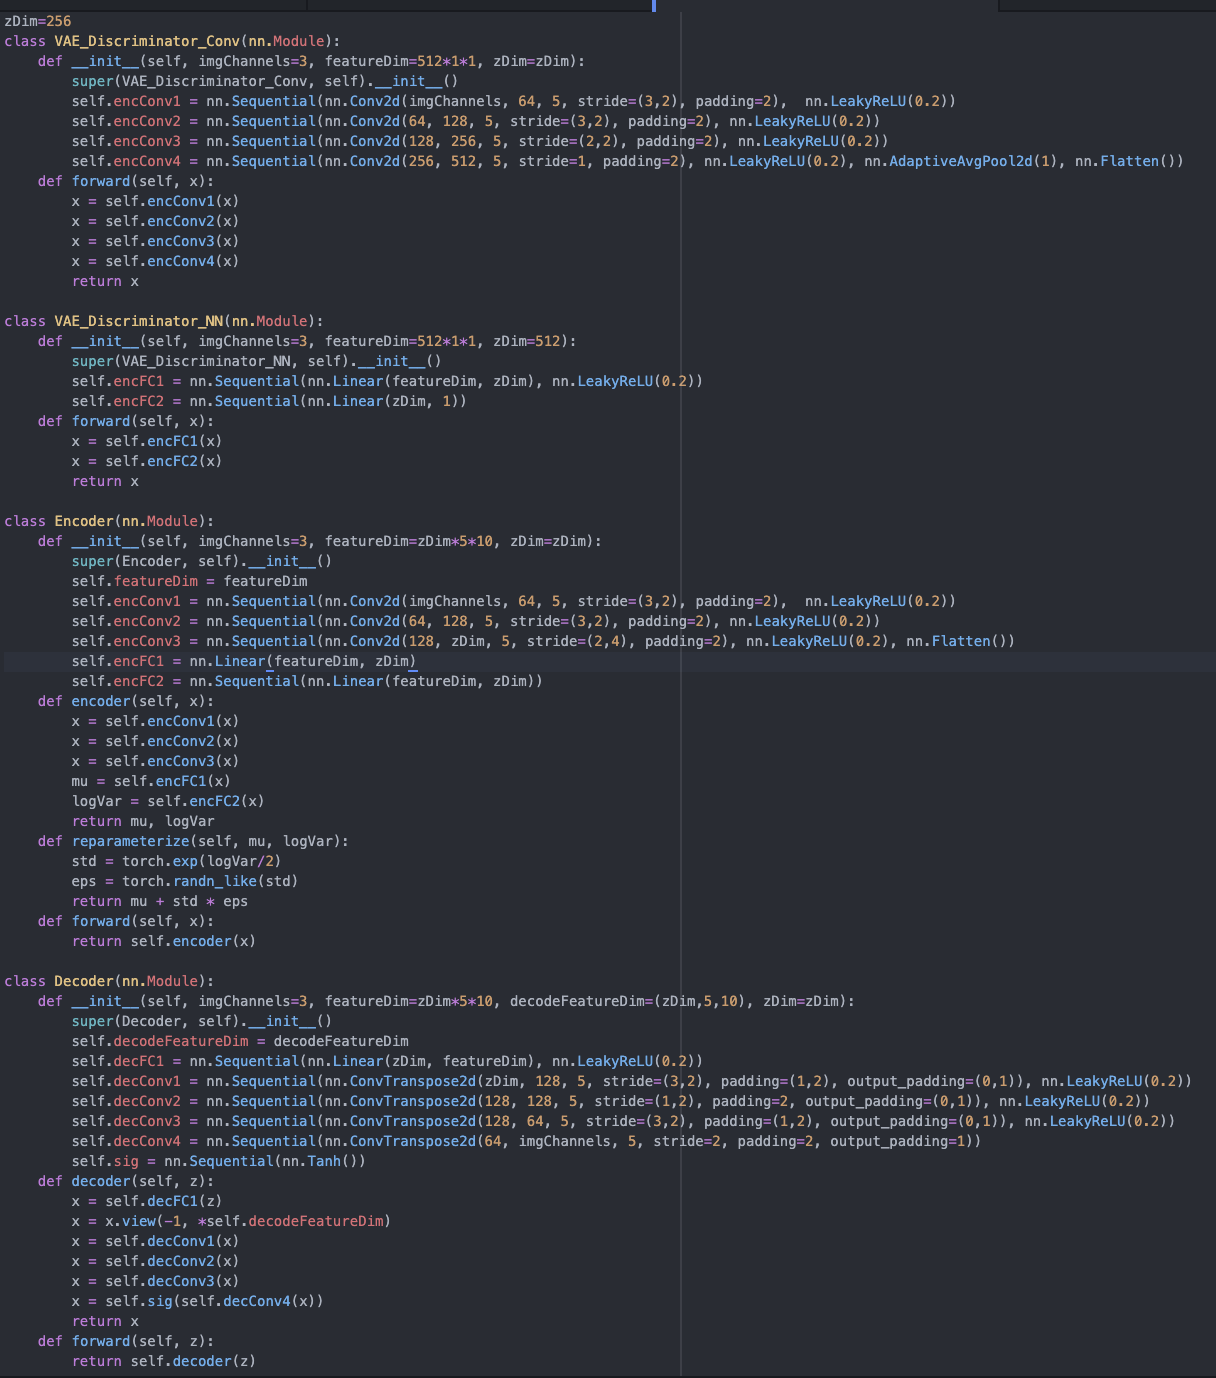
\includegraphics[scale=0.5]{model1.png} \\
This model was trained with a learning rate of 0.00001, and a batch size of 256, for 500 epochs, using image sizes of (3,90,160). This resulted in the following test image pairs (left column is input images, and right column is the reconstructed image from the decoder): \\
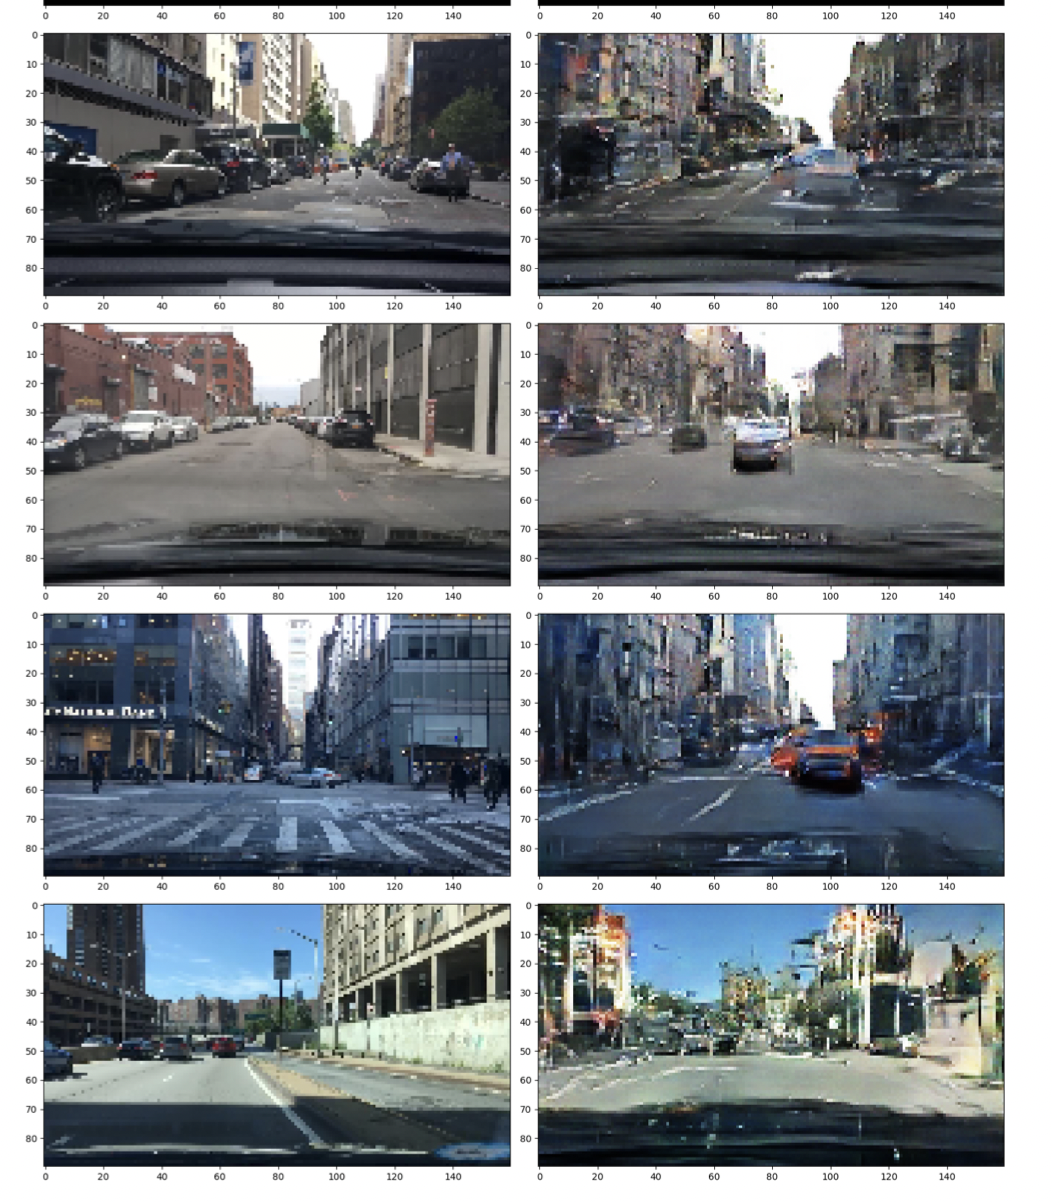
\includegraphics[scale=0.5]{results1.png} \\
While far from perfect, this is highly promising, and much more in line with what appeared in the original comma.ai paper. However, there is a severe degree of mode collapse in the reconstructions - many high level details are superficially similar, but many key details within the scene are dangerously wrong - vehicles where there shouldn't be any, and more. This clearly shows that such an encoding is highly likely to be in mode collapse, and thus, not very useful for an end-to-end AV controller.
\subsection{Model regularization and simplification}
Thus, the following final revisions to the beta-VAE-GAN model were done as follows:
\begin{enumerate}
    \item To support making far less aggressive and irregular strides as previously, we changed the size of the images in question from (3,90,160) to (3,128,128). This allows us to merely use strides of 2 at each encoding and decoding layer.
    \item We switched to using a library called torchgan to standardize our model creation - however, loss functions were kept exactly the same.
\end{enumerate}
This new model scheme's python code is also presented here, and is present in the github code attached: \\
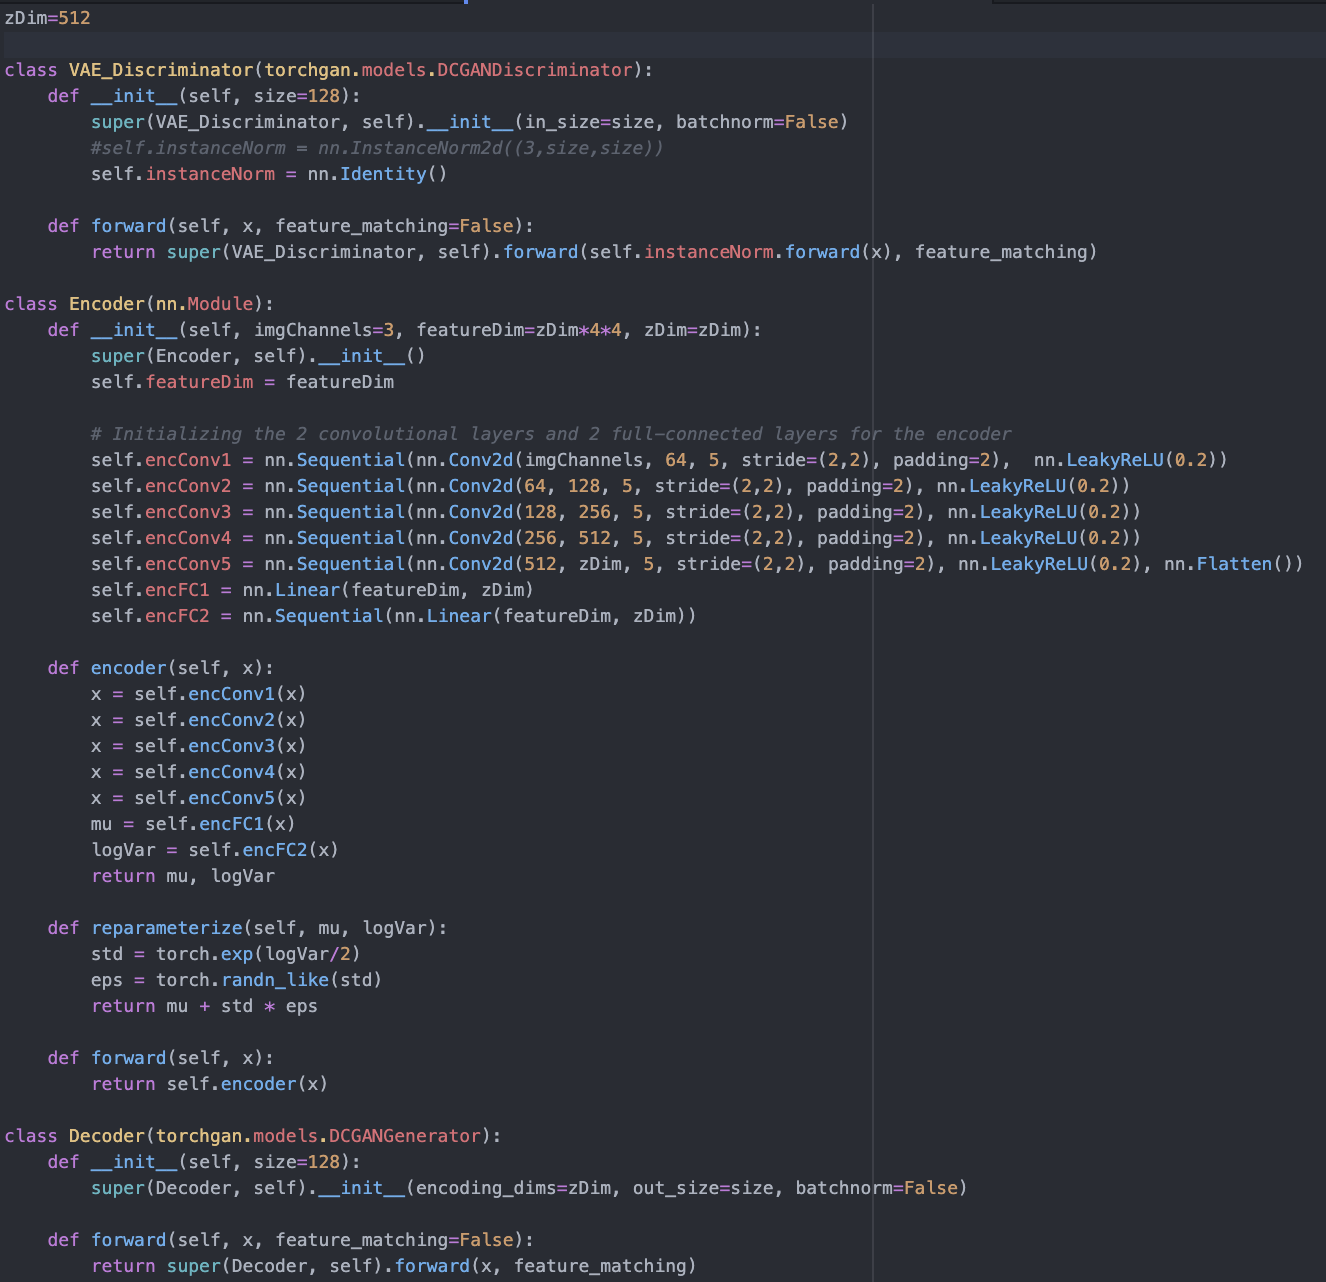
\includegraphics[scale=0.5]{model2.png} \\
This model is trained with a learning rate of 0.00002, a batch size of 512, for 72 hours, or approximately 750 epochs. 
With a beta of 1, this GAN approach appears to produce promising results with less apparent mode collapse: \\ 
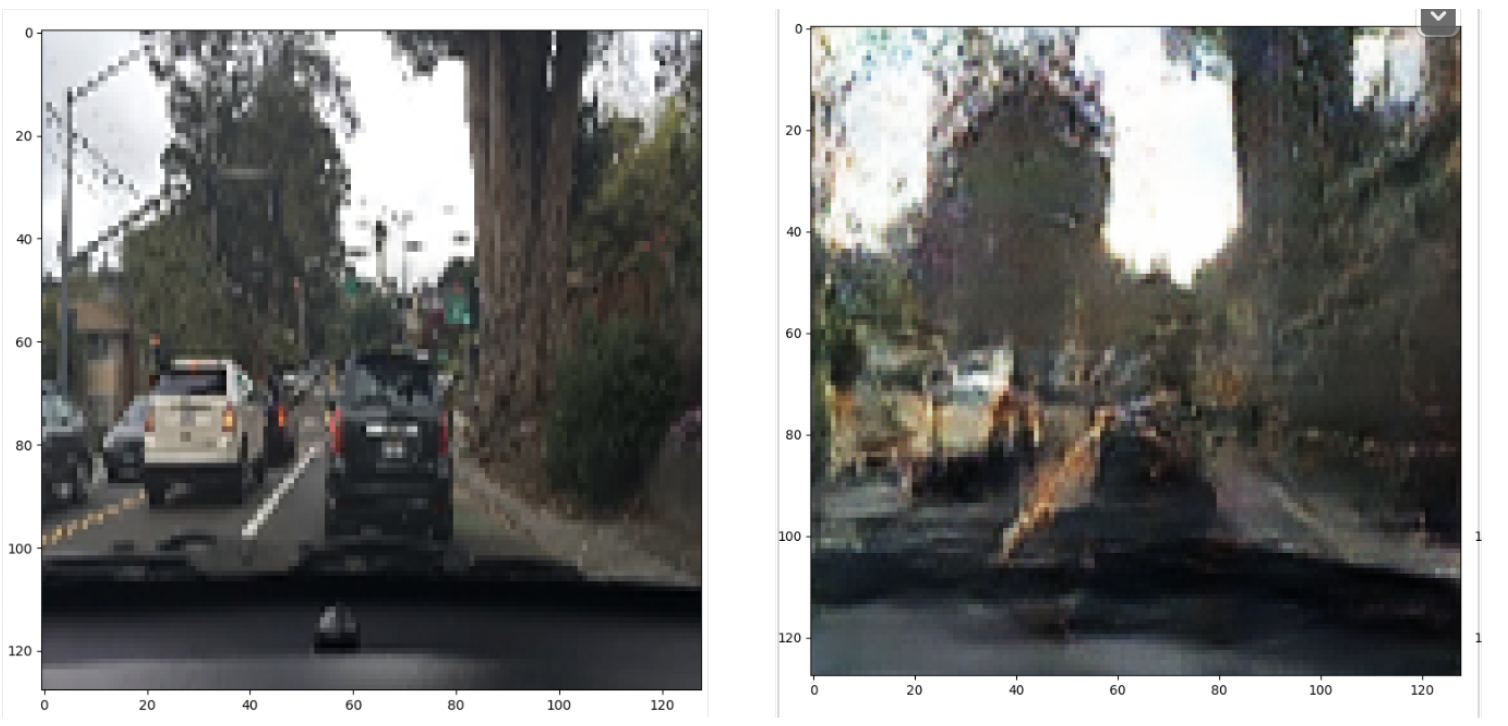
\includegraphics[scale=0.5]{results2.png} \\
As one can see here, more local features are preserved in this new model approach, and mode collapse is not as overtly subjectively apparent as before. However, this still doesn't indicate how entangled the latent space variables are. In order to do this, we must perform a sweep of each latent variable, using an encoding created from a "seed" image, to see what changes to each individual latent variable do to the image itself. Ideally, a latent variable sweep should change one single aspect of the image, and not result in a complete transformation of the entire scene (which would indicate entanglement with the scene as a whole). This would also allow us to validate or disprove our second hypothesis w.r.t. this end.
\section{Beta Hyperparameter Experiment}
To this end, we trained four models with a beta hyperparamter of 1, 10, 100, and 250 respectively. These models are trained with a learning rate of 0.00002, a batch size of 512, for 72 hours, or approximately 750 epochs. We then used the previous dashcam image that was compared with its reconstruction in section 3.5 as a baseline that we use to create our latent encoding "seed." For each latent variable, we create a row of 11 images where we sweep around the seed's value for that variable - the leftmost image column is at that latent variable's original value minus 50, with the column's value for that latent variable increasing by 10 at each next column step, until the 6th column, which is at the latent variable's original value. All other latent variables in the encoding are left unchanged for each row. For each beta hyperparameter, two latent variable sweeps are shown to illustrate how the scene typically changes for a latent variable sweep across all 4 beta hyperparameter configurations. This code is available on the github page for more rigorous, close examination.
\subsection{Beta = 1 (Normal VAE-GAN)}
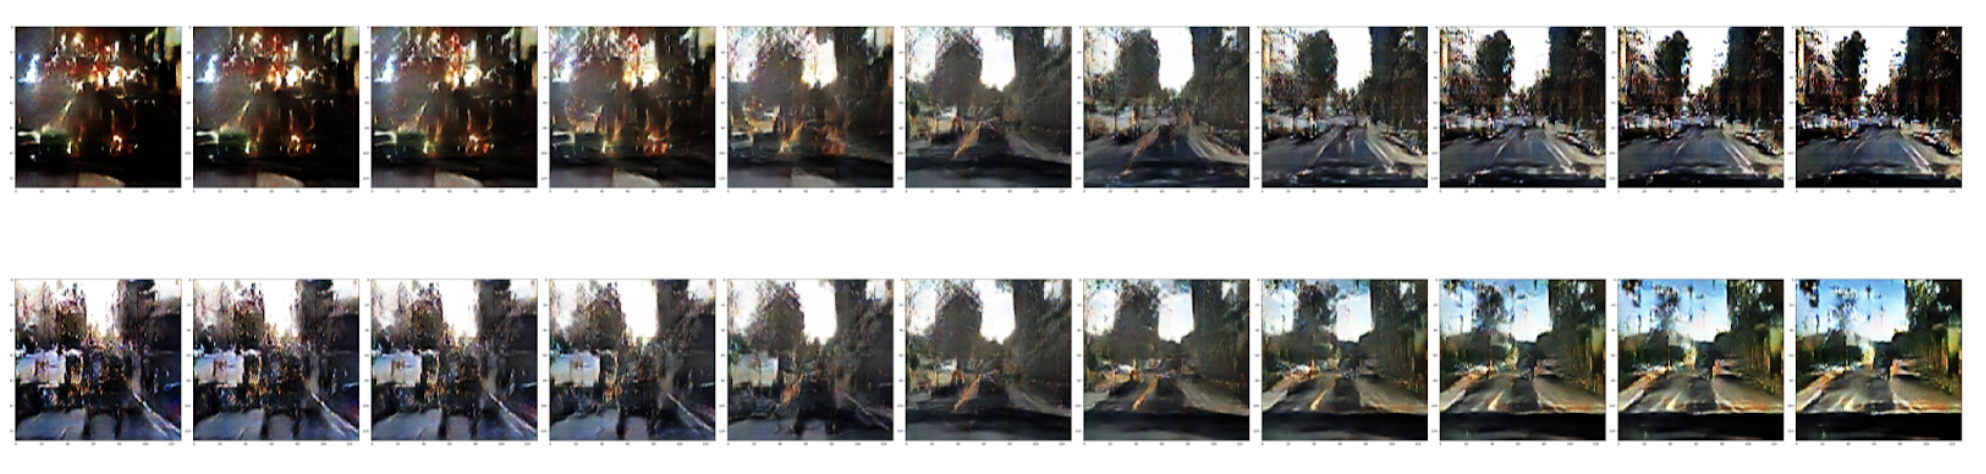
\includegraphics[scale=0.5]{resultBeta1.png} \\
\subsection{Beta = 10}
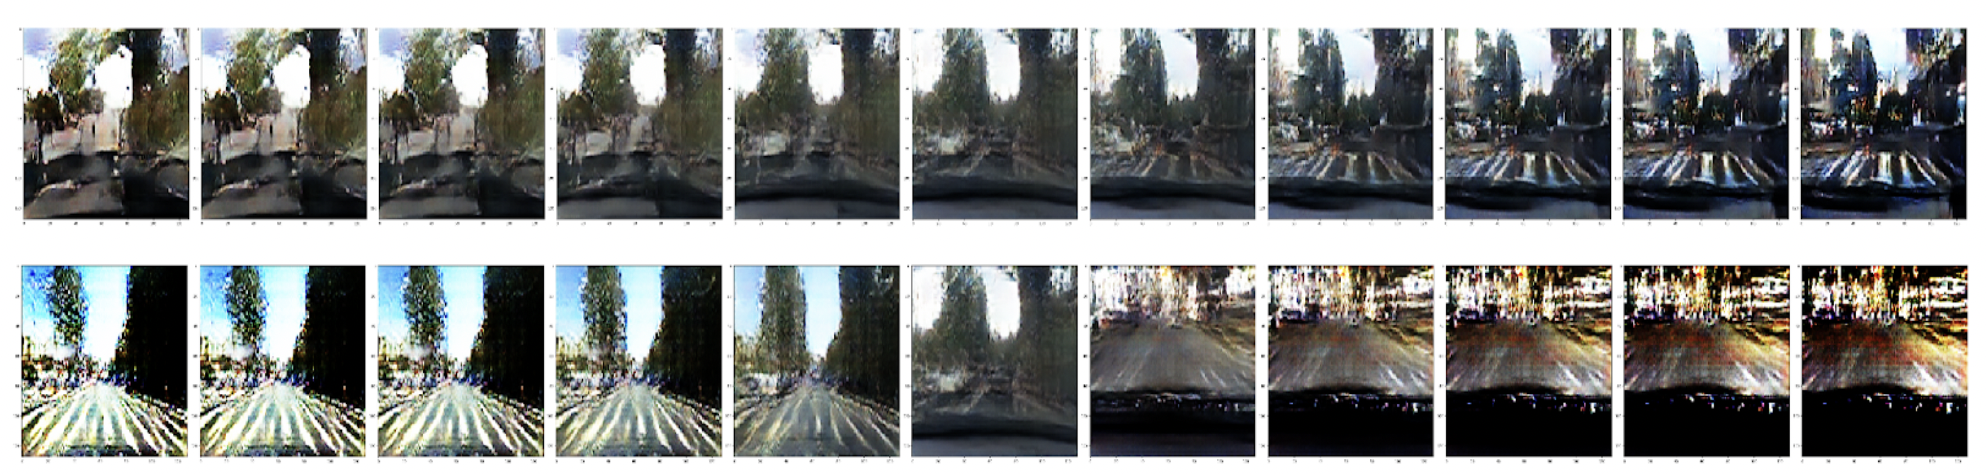
\includegraphics[scale=0.5]{resultBeta10.png} \\
\subsection{Beta = 100}
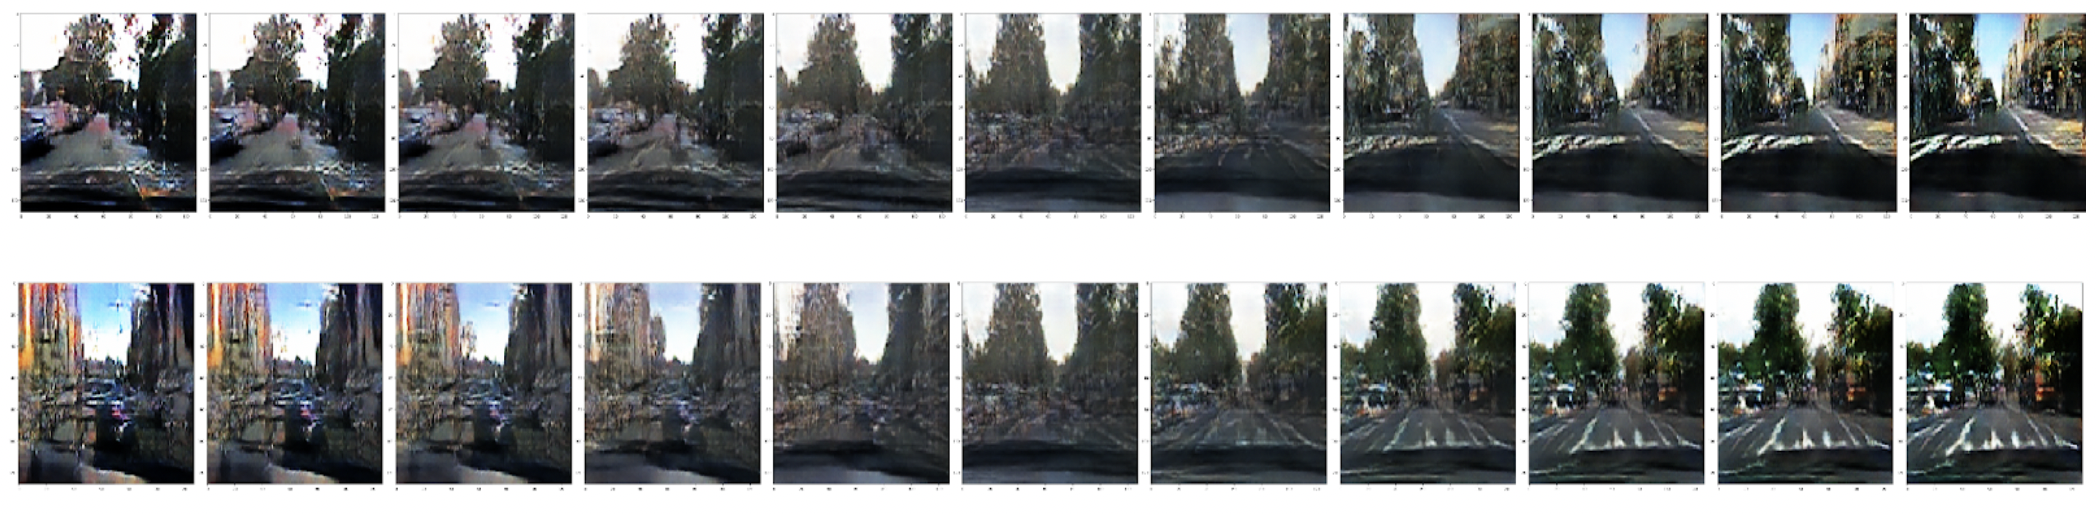
\includegraphics[scale=0.45]{resultBeta100.png} \\
\subsection{Beta = 250}
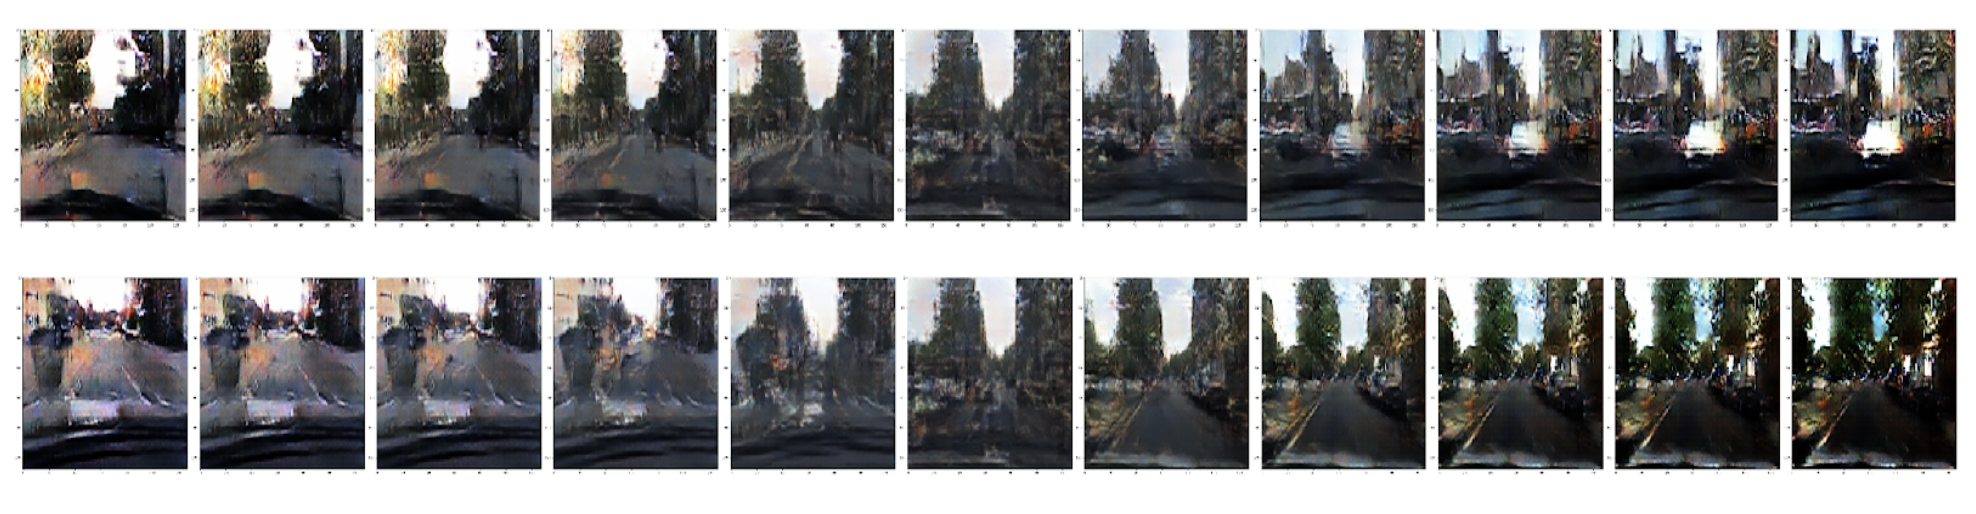
\includegraphics[scale=0.5]{resultBeta250.png} \\
\subsection{Experiment conclusion and summary}
In terms of not disproving our second hypothesis, this experiment appears to be a failure - it seemingly appears to disprove it. Changing one latent variable by a large degree, either in a negative or positive direction, is more than enough to completely transform the scene. This is true across all 4 beta hyperparameters. The shown images above are representative of the behavior of the latent variable encodings at each hyperparameter. Quite tellingly, at the extreme ends of the variable sweep (-50 or +50), we see highly distinct scenes - it's possible that these represent the modes that the latent encoding has learned. Even though the images become significantly blurrier at higher beta hyperparameters, it appears to do little to alleviate the entanglement inherently involved in the encoding itself. In summary, with our current models, hypothesis 2 is disproven, and there is not a clear path forward towards alleviating this problem. 
\section{Discussion}
This work appears to show that this initial phase of our overall end-to-end AV controller project has been a failure. While we are able to create an encoding-decoding model that provides an excellent start that provides a reconstruction of many local features of an image, the latent encoding appears to be highly entangled. This would make such a latent encoding a bad input source for an AV controller, such as Comma.Ai's transition model - it likely would not obtain as high of an accuracy as it would with a properly disentangled latent space input. While it's still subject to speculation, we speculate that the beta-VAE-GAN has seemingly associated each latent variable with an image/"scenario" that it has inferred from the dataset indirectly via the discriminator. This would explain why large changes to an individual latent variable appear to create highly detailed and crisp images that are clearly distinct from the image that is supposed to be reconstructed. It's possible that a longer training time than 3 days would see this problem be reduced to some extent, but time constraints prevent further exploration of this. \\ 
Another aspect of this problem to keep in mind, especially compared to GANs trained on human faces or handwritten digits, is that dashcam footage has considerably more information encoded in it, and different in nature. Dashcam footage has a high amount of objects with very dynamic spatial profiles - cars, pedestrians, and other such objects can appear at many different spots of the image, whereas in images such as faces and digits, many visual aspects stay in relatively the same location. It's a fancy way of saying that this problem is drastically harder than many state-of-the-art problems currently being studied!
\section{Future plans}
It's not clear what the future path is going forward, but there are many promising alternatives. One thing to keep in mind is that the model architecture used in this work is relatively old - Deep Convolutional GANs are several years old at this point, and our model does not use any residual connections, minibatch discrimination or other such "modern" augmentations. Furtermore, it might be possible to just train the models for a longer time as well - such as 2 weeks. Many works in the GAN field train their models for longer than a few years, unlike us, who at most trained our models for 72 hours for time constraints. \\ \\
We have a long-term perspective on this project, and thus early failure like this to some degree was expected. It's anticipated, with some measure of hope, that persistence and continued exploration of GAN technologies will provide continued improvement and performance. Already in this work we have achieved considerable progress - in the beginning we could not create a model capable of training at all! Now we have a model that can train and produce a reconstruction that at least resembles what the original encoded image was. It would be pessimistic to assume that we have come remotely close to exhausting all of the augmentations and additional approaches to this problem. \\

We're excited to continue this work and make further improvements, with an aim that is still aimed towards creating an end-to-end AV controller based on this concept.
\bibliographystyle{ACM-Reference-Format}
\bibliography{sample-base}

\end{document}